\chapter{Introduction}
\label{chap:Introduction}
\index{Introduction}

%%%%%%%%%%%%%%%%%%%%%%%%%%%%%%%%%%%%%%%%%%%%%%%%%%%%%%%%%%%%%%%%%%%%%%%%%%%%%%%%

In this chapter, we will first introduce our team's previous work named Illimitable Space System (ISS) then point
out the pain spots we encounter when using it.
Motivated by these issues, we propose the goal we would like to
achieve in this thesis.
Furthermore, we define our research problems and extract
requirements from usage scenarios.
Finally, we discuss our contributions, followed by a brief introduction
to each of the following chapters.

\section{Background}
\label{sec:intro-background}

Due to our previous work~\cite{iss-v2-design-theory-journal} named ISSv2, we
were able to create real-time motion capture, projection mapping and artistic
performance on the stage with one camera. Some example images of our
performance are shown as~\autoref{fig:bg}.

\begin{figure}[ht]
    \begin{subfigure}
        \centering
        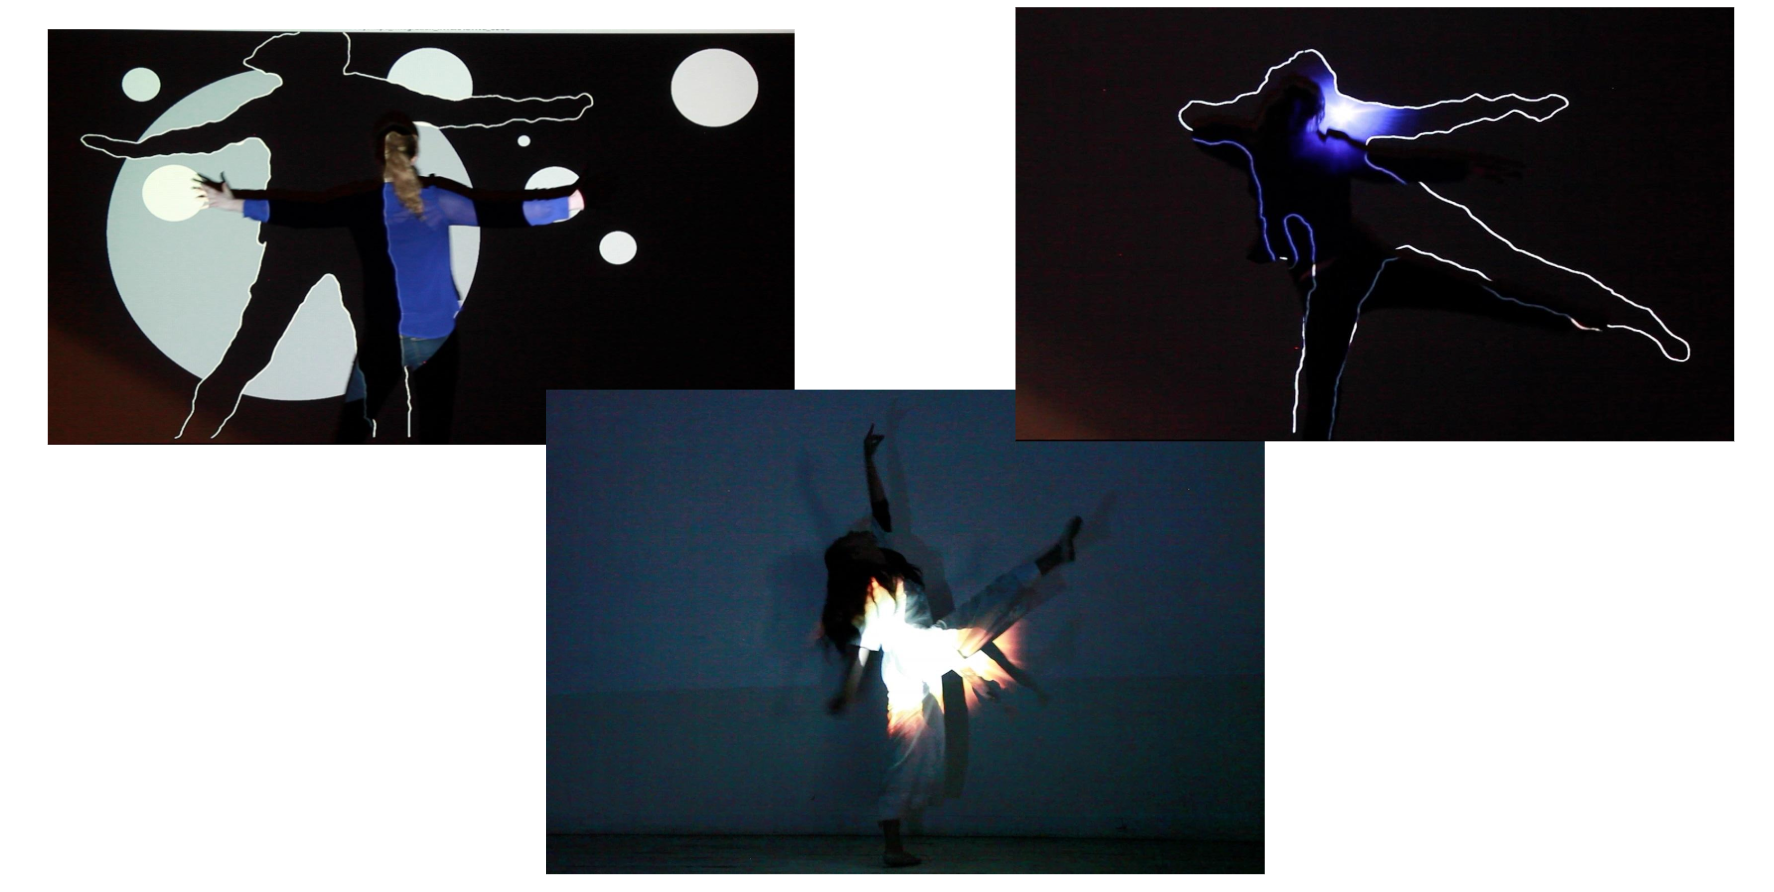
\includegraphics[width=.8\linewidth]{figures/bg1.png}
        \label{fig:sub-first}
    \end{subfigure}
    \begin{subfigure}
        \centering
        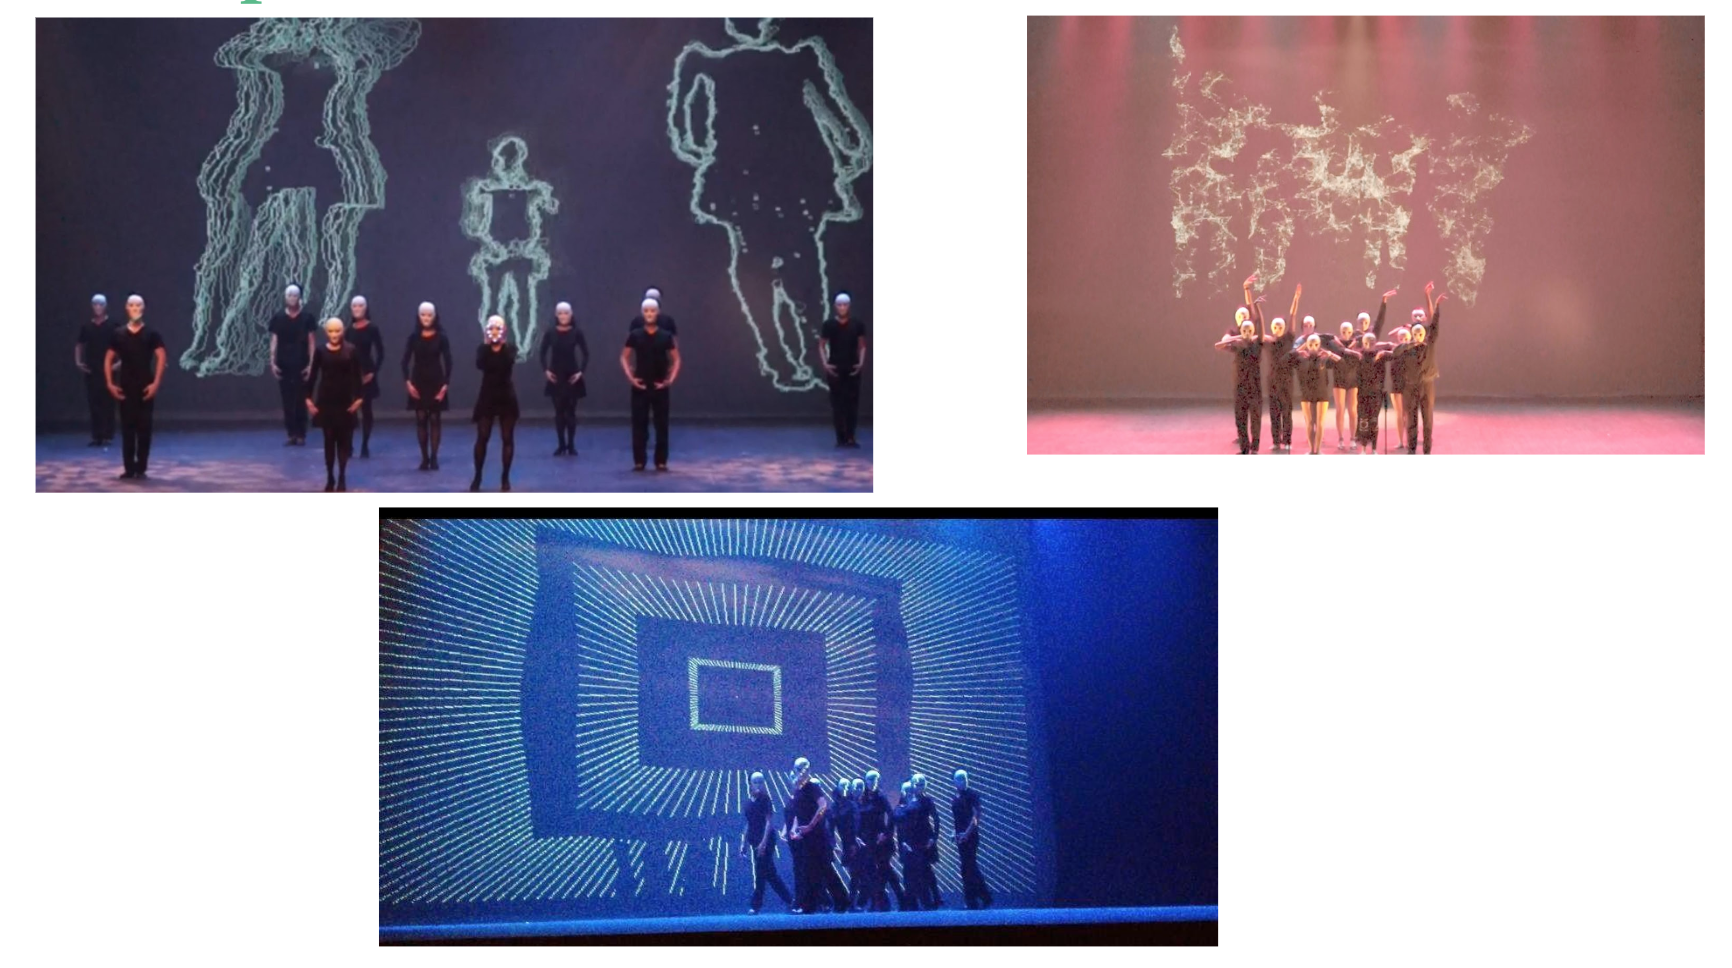
\includegraphics[width=.8\linewidth]{figures/bg2.png}
        \label{fig:sub-second}
    \end{subfigure}
    \caption{Artistic show produced by ISS}
    \label{fig:bg}
\end{figure}

\begin{figure}
    \begin{center}
        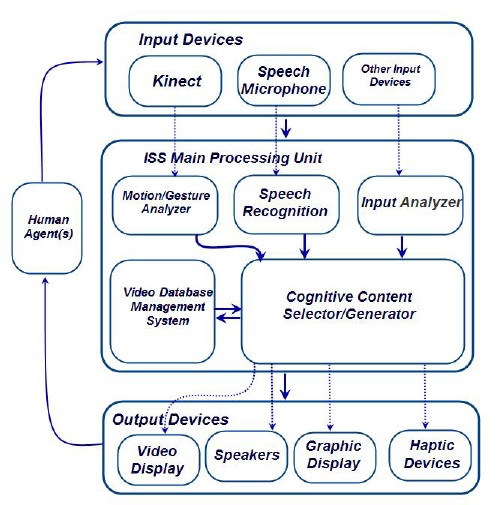
\includegraphics[scale=0.6]{figures/iss_v2_model.png}
    \end{center}
    \caption{Block Diagram of Illimitable Space System}
    \label{fig:iss-v2}
\end{figure}

ISS (Illimitable Space System) is a real-time interactive configurable
artist's toolbox used to create music visualizations, visual effects and
interactive documentary based on the inputs from users such as gestures or
voice.
The goal of ISS is to enhance interaction between actors and graphics so that
it is all projected as an integrated piece. It aims at freeing up the artists
as much as possible so that they are able to perform freely in their own way
without worrying about the performance technology.
ISS was originally proposed in~\cite{first-proposed-iss} and improved 
in~\cite{iss-v2-design-theory-journal}, in order to differentiate them, we named
the former ISSv1 and the latter ISSv2. Also, there was 
ISSv3~\cite{iss-v3-appy-hour-gem2015, iss-v3-appy-hour-siggraph2015} which
was designed for virtual reality application, but out of this thesis scope. We
mainly focus on ISSv2 which can be conceptually represented by~\autoref{fig:iss-v2}, 
which is a significant improvement in ISSv1 and is used
for rapid development of real-time, motion-based graphics applications
implemented in Processing which is on top of Java.

\section{Limitations of ISSv2}
\label{sec:intro-lim-issv2}

When we have more chances to do different performances in different places,
we found that sometimes the stage given to us is too large and cannot be covered
by only a single camera. It restricts us to design the performance within a
limited space, which is actually conflicting with our project's name, Illimitable Space
System.
Also, recently the price of consuming level depth camera has become
much cheaper. In the market, there are different kinds of depth cameras
being manufactured (like Kinect v1, Kinect v2 and RealSence) and these cameras
become more and more powerful (higher speed, frame rate, resolution, larger
bandwidth and etc). But ISSv2 is hardware-dependent can only work with Kinect
v1 which is kind of out of date now.

Under such a situation, we started to think that if one camera is
not enough, we can have more than one and each of them takes care of a certain
area of the large stage so that we break the restriction and can design much
better performance without space limitation.
By using more than one camera, a problem comes to our mind naturally: How can
we identify the same person across different cameras since we need to track them
and apply specific visual effects on certain actors?
From this point, developing a system that can track people through multiple
cameras becomes essential.
This idea can not only benefit us but also the security-and-protection industry
or even the police department. Since with such a system, you can identify a
specific target (like suspect) across multiple cameras if you have captured it
in any one of your cameras.

In order to catch up with the device evolution, we would like to move from 
older devices to the latest models. But we don't want to discard our previous 
compatibility while evolving to new technologies. So how to enable our previous work to be 
compatible with various kinds of cameras is also a challenge for us.

%\section{Problem Statement}
\section{Research Problem}
\label{sec:intro-pbstat}

%In order to address the limitations we found for ISSv2, our research can be

From the situation we described above, our research can be
intuitively divided into two parts: 
(1) person re-identification and
(2) depth camera abstraction.
Person re-identification (ReID) recently is a hot research topic in the
computer vision community. It requires the system to identify the same person
across different cameras, which can be broken down into three components:

\begin{itemize}
    \item person detection
    \item person tracking
    \item person retrieval
\end{itemize}

If we have a fast enough system, we don't explicitly need person tracking.
Instead, we perform person detection on each coming frame from the camera which
is functionally equivalent to person tracking. Under this consideration, we
omit person tracking in this thesis.
For device encapsulation, we  currently focus on the total of three kinds of
cameras: Kinect v1, Kinect v2 and RealSense D435 and we also make sure that when
a new device needs to be appended, the process will be simple and
implementer-friendly as well as having no side-effect with the existing devices.

In the following subsections, we are going to formulate our
research problem scientifically. For person detection, we enlarge our target
set not only on the person but for all kinds of objects and the same applies to
person retrieval. So we end up with object detection and object retrieval.

\subsection{Object Detection}

In object detection, you are given an image $I$ and a list of classes $C$ which
the objects
appear in $I$ belong to. Your task is to detect instances of the object within
$I$ belong to a specific class in $C$.
For each instance $i$, you need to output first $c \in C$ which represents which class
this instance belongs to and second
a bounding box $B$ to indicate the location of that instance with respect to the
image $I$.

\subsection{Object Retrieval}

In object retrieval, you are given a query image $q$ and a set of gallery images
$G$. Your task is to find the
most likely image $g \in G$ for which both $q$ and $g$ represent the same instance
$instance(q) = instance(g)$.

\subsection{Device Abstraction}

The second part we mentioned above is that we try to conceptually eliminate the differences
among various kinds of cameras. It can be translated as we would like to access
data via a set of common APIs without considering what kind of hardware
we are using. Assume we have a list of device $D = {d_1, d_2, ..., d_n}$ and a
list of API $F = {f_1, f_2, ..., f_n}$,
we can trigger the same effect
while calling the same API which can be mathematically expressed as:
$
\exists f_n \in F, \forall (d_i, d_j) \in D
\Longrightarrow f_{n}(d_i) = f_{n}(d_j)
$

\section{Motivation and Goal}
\label{sec:intro-mot-goal}

The original design of ISSv2 targets to create music visualization, visual
effects and interactive documentary easily for artistic people who don't have 
extensive knowledge in computer science and programming. So the architecture and
the design needs to be relatively simple. The main focus should be given to visual effect
design and how to display them to the audiences.
What's more, currently, ISSv2 can only use Kinect v1 as the input device. Efforts have
been put to enable Kinect v2 but due to the low-level dependencies (e.g.
hardware driver) conflict, not all the features can be replicated and compatible.

Based on the limitation we found and some new demands,
we conducted a comprehensive survey and found that there is no existing solution
targeting our problem directly.
So we would like to abstract a back-end system for ISS while keeping the
front-end remaining unchanged. The back-end system here means the hardware,
scheduling algorithm, pipeline construction, and other common APIs. Front-end
basically means the artistic part, like visual effect design, music
visualization and so on.

It is worthwhile to mention that as this work is being developed, there are
another two other research works going on in parallel under the same umbrella.
Jashanjot Singh is working on a system that can do gesture tracking and
recognition while Yiran Shen is working on a system that can do facial
landmarks detection and facial expressions recognition. We would also like
these two works to be accessed via the same set of APIs which means all these
three works should somehow be operated within the same operational software
framework.

Up to now, we should be able to summarize our goal:
\textbf{
    we would like to design and implement a system that provides a way to
	abstract different kinds of depth cameras and the functionality of person
	re-identification. It should also leave space for other modules to be
	integrated with good extensibility and usability.
}

\section{Scenario and Requirement}
\label{sec:intro-scen-req}

With the goal we defined above, in this section we will give a few concrete
use-case scenarios we expect to achieve from the final production of this thesis.
These scenarios, in their own way, highlight one or more problems that have not
been solved by any existing solution yet. We not only aim at solving these problems
individually, but also to provide a general solution to all these problems
under the same software solution.
We analyze these scenarios one by one, then extract both functional and
non-functional requirements, which becomes the concrete implementation goal of
our solution.

\subsection{Device Switch and New Device Addition}
\label{sec:intro-sq-dev}

Imagine a scenario where we would like to develop a new version of ISS
may be named ISSv4. This time, we need to support device $D_1$ and $D_2$ where
$D_1$ was supported by its previous version and $D_2$ is a newly added device.
The difference between $D_1$ and $D_2$ is that $D_1$ was designed for the indoor
environment while $D_2$ can perform better in the outdoor environment. So depending on
where the performance will be given, we need to be able to switch between $D_1$
and $D_2$. This kind of switch should just literally unplug one device from
the system and plug in the other one. Only a few or even no modifications should
be made in the code to obtain the same effect from the application point of
view. Also, if later a new device $D_3$ comes to the market, the system
should be easily extended to be able to make use of $D_3$.

This usage scenario can be abstractly summed-up as the following, which becomes
two of our requirements:

\begin{itemize}
    \item \textbf{FR1}: The solution shall provide an abstraction layer for the
    hardware that enables the physical device transparency property to
    the users.
    \item \textbf{FR2}: The solution shall ensure the extensibility of the
    abstraction layer required in \textbf{FR1} which means when the new devices
    come only a few or no modification need to be made and will not affect the
    existing system.
\end{itemize}

\subsection{Back-end Abstraction}
\label{sec:intro-sq-abs}

Let's continue using the scenario setting we described above, this time we need
to map the performance onto another backdrop rather than the one where the
actual performance is taking place, which means that we need to extract only
the actors out with all the other background removed. Keep in mind that
there are two different devices supported $D_1$ and $D_2$, according to our
settings. The most straightforward way to do is that for each device, we
create a filtering algorithm employing some methods provided by the hardware
driver to perform background removal. But the limitation is also obvious when
a new device is added: you have to re-implement the same algorithm again and
again for each new device. If another demand is required, you need to implement all of them when a
new device is being supported.
Another elegant solution is that we could extract the data needed to perform
background subtraction into a common data structure then apply a general
algorithm based on it. Next time, when a new device comes, what we need to do
will be just the transformation from the device-specific data structure to our
common one. If some other demands like background removal are required, we can
always follow the same pattern to solve them. We call all these common data structures
and common algorithms the back-end of the system.

This usage scenario can be abstractly summed-up as the following, which becomes
one of our requirements:

\begin{itemize}
    \item \textbf{FR3}: The solution shall be able to serve as a back-end of the
	existing ISS system providing a set of commonly used data structures and
	functionalities for reusability.
\end{itemize}

\subsection{Person Re-identification}
\label{sec:intro-sq-reid}

Imagine a scenario where there is a show given by two actors, and we would like to
project visual effect $\mathit{vfx}_1$ on actor $a_1$ while $\mathit{vfx}_2$ on
actor $a_2$.
Unfortunately, the stage is too large and cannot be covered by a single camera.
We have to employ two cameras, each of them covers half the space of the stage.
According to the performance director, we need to make sure that no matter
where these two actors are, the visual effects have to be mapped properly.

This usage scenario can be abstractly summed-up as the following, which becomes
one of our requirements:

\begin{itemize}
    \item \textbf{FR4}: The solution shall be able to detect all the appearance 
    of human bodies and provide their location by bounding boxes.
    \item \textbf{FR5}: The solution shall be able to recognize a cropped image 
    with an identity across multiple cameras if the identity has been defined in 
    advance.
\end{itemize}

\subsection{Skeleton Tracking}
\label{sec:intro-sq-skt}

In ISSv2, we have some visual effects designed specifically for the human 
skeleton. But because of the underlying dependencies issue, we can only obtain 
the skeleton data from Kinect v1 camera.
In order to break the restriction from the specific device-oriented
dependencies, we need to make the skeleton extraction process 
device-independent.
It means we should be able to extract skeleton data from a variety
of devices and convert them into the common skeleton data format which is simply 
a set of points in a picture. A possible scenario can be described as the following: a
performance director would like to make use of some skeleton-based visual
effect and want them to be used with different devices.

This usage scenario can be abstractly summed-up as the following, which becomes
one of our requirements:

\begin{itemize}
    \item \textbf{FR6}: The solution shall provide the functionality to enable
    users to perform skeleton tracking among various kinds of cameras.
\end{itemize}

\subsection{Interaction with Other Modules}
\label{sec:intro-sq-inta}

As mentioned before, there are a gesture and facial recognition modules being developed
concurrently to our research. Theses modules should be able to use the infrastructure (e.g.
device abstraction) we proposed in this thesis. Also the module we develop here
should be able to communicate with these two other modules from other system
developers. Imagine a scenario where the visual effect needs to change according
to the actor's gestures. When the actor push their hand, a zoom-out
effect should be applied while the actor pull their hand, a zoom-in effect
occurs.

This usage scenario can be abstractly summed-up as the following, which becomes
one of our requirements:

\begin{itemize}
    \item \textbf{FR7}: The solution shall provide fundamental infrastructure
    for other modules to use and vice versa. It shall enable an abstract 
    communication infrastructure common to all developed modules.
\end{itemize}

\subsection{Non-functional Requirements}
\label{sec:intro-non-func-req}

By analyzing the scenarios we described previously, we found that in order to
achieve them our solution must meet the following non-functional requirements:

\textbf{Extensibility:}
\textit{The ability of a software system to acquire and integrate new
components.}

As the devices will become more and more multitudinous and the algorithms for
person re-identification will be more and more advanced, it becomes essential
to design a solution with great extensibility that later on we still
be able used to add or integrate more devices and algorithms into our existing
solution smoothly and easily.

\textbf{Usability:}
\textit{The ability of a software system to effectively provide the expected
functionalities to the user, in a manner that is as intuitive and the least
strenuous or
problematic as possible.}

For any kind of software system, in order to attract the users and/or programmers, as the designer
we should try our best to provide simple, meaningful and understandable APIs.
That means the name of our APIs, the required parameters for each functionality
and the final result from the return value should be concise, compact and
logically make sense. For the experienced users in the same area, they should
be able to move from other similar solutions to ours without putting too much effort.
In other words, the learning curve should be as smooth as possible
and necessary documentation and comments should be provided properly.

\section{Contributions}
\label{sec:intro-contrib}

Our contribution are four-fold:

\begin{itemize}
    \item We offer an overall architecture that allows users to perform
    real-time skeleton tracking, person detection, and person
    re-identification.
    
    \item We offer a way in general that can allow the user to access
    different depth cameras within the same set of APIs with good extensibility.
    
    \item We offer a way to allow cross cameras tracking with a pluggable
    detector and recognizer.
    
    \item We offer a pipeline execution mechanism to allow the user to assemble 
    various components to form their application without knowing the underlying 
    details.
    
    \item We offer a way for the researcher to enable person re-identification
    experiment on top of TensorFlow and Keras.
\end{itemize}

\noindent To achieve the above, we implemented the following features:

\begin{itemize}
	\item Design and implement a modular framework solution which consists of
	the core and specialized frameworks that enable real-time skeleton 
	tracking, person detection, and person re-identification.

    \item Design a device module that encapsulates the depth cameras from
    different brands with good extensibility. Instantiate this module to
    support three kinds of physical devices.
    
    \item Design and implement a pipeline module that provides a linear
    execution mechanism over a series of filter that each encapsulate a 
    specific transformation step.

    \item Design a detector specialized framework and instantiate it for
    person detection task with a deep learning-based algorithm named YOLO.

    \item Design a recognizer specialized framework and instantiate it for
    person re-identification using the deep learning-based identification and
    triplet models.

    \item Use the general framework solution to build several commonly used
    applications like camera calibration, green screen image, and image
    alignment.

    \item Implement an abstraction layer for deep learning-based person
    re-identification dataset to allow training and validation among multiple
    dataset easily.
\end{itemize}

%\section{Methodology}
%\label{sec:intro-methodology}

\section{Thesis Outline}
\label{sec:intro-outline}

In this chapter, we introduced our research background, pointed out the
existing limitations, and stated the research problems giving them clear academic
definitions and restricted our scope.
In the following chapters, the thesis will be structured in the way listed
below:

\begin{itemize}
    \item In \autoref{chap:RelatedWork}, we will review existing literature
    related to our research problem and also the available software which is
    useful for our implementation. In the summary section of this chapter,
    based on our need, we will select our target detector and recognizer and
    stick with them in our implementation described in the following chapters.

    \item In \autoref{chap:fw-design} and \autoref{chap:fw-inst}, with all
    needed background in hand from the previous chapter, we will propose our
    solution in detail and explain our design and implementation in a top-down
    manner.

    \item In \autoref{chap:fw-app}, we will describe the applications built on
    top of our proposed solution, which becomes a proof of concept that our
    solution can actually fulfill our functional requirements.

<<<<<<< HEAD
    \item In \autoref{chap:Evaluation}, we will report our results showing the
	benchmarks for the main components in our solution with commonly acknowledged 
	metrics. Also, we will prove that both functional and non-functional
    requirements are really fulfilled.
=======
    \item In \autoref{chap:Evaluation}, we will first demonstrate both the
    functional and non-functional requirements are really fulfilled by our
    framework solution. Then we report our result showing the benchmark for the
    main components in our solution with commonly acknowledged metrics.
>>>>>>> 8a860f413a6d6a177b30d175dd449d3f0ea1566b

    \item In \autoref{chap:Conclusion}, we sum up our work with advantages and
	limitations and point out some potential research directions in the future.
\end{itemize}

%In the following chapters, we will first describe the existing solution of our
%interested research and review corresponding literature in
%\autoref{chap:RelatedWork}
%so that we can see the gap and understand the current state of the art in this
%domain.
%With all needed background, we then will propose our solution in detailed and
%explain our design and implementation in a top-down manner in
%\autoref{chap:fw-design} and \autoref{chap:fw-inst}. Followed by the
%application we built on top of our solution to address the cross cameras
%tracking problem \autoref{chap:fw-app}.
%In \autoref{chap:Evaluation}, we will report our result showing benchmark for
%each components in our solution with commonly acknowledged metrics.
%At the end, we sum up our work with advantages and limitations, pointing our
%some potential directions for future work \autoref{chap:Conclusion}.

% EOF
